\documentclass[10pt]{beamer}

\usetheme{Oxygen}
\usepackage{thumbpdf}
\usepackage{wasysym}
\usepackage{ucs}
\usepackage[utf8]{inputenc}
\usepackage{pgf,pgfarrows,pgfnodes,pgfautomata,pgfheaps,pgfshade}
\usepackage{verbatim}
\usepackage{tikzsymbols}

\usepackage{ragged2e} % maneja la alineación del documento
\usepackage[spanish]{babel} % Títulos en español
\usepackage[utf8]{inputenc}
%\usepackage[latin1]{inputenc} % Caracteres con acentos.
\usepackage{graphicx} % Soporte para gráficos
\usepackage[none]{hyphenat} % indica a LaTeX que no debe hacer partición de palabras
\usepackage[T1]{fontenc} % manejo de fuentes
\usepackage{array}
\usepackage{amsmath}
\usepackage{amssymb}
\usepackage{float}
%\usepackage{ra  gged2e}
\usepackage [all]{xy}
\usepackage{lmodern}
\usepackage{multirow}
\usepackage{multicol}
\usepackage{tikz}
\usepackage{listings}
\usepackage{longtable}

\lstset{keywordstyle=\color{blue}, 
commentstyle=\color{gray!90}, 
basicstyle=\ttfamily\scriptsize, 
columns=fullflexible, 
breaklines=true,
linewidth=\textwidth, 
backgroundcolor=\color{gray!20}, 
basewidth={0.5em,0.4em}, 
literate={á}{{\'a}}1 {ñ}{{\~n}}1 {é}{{\'e}}1 {ó}{{\'o}}1 {º}{{\textordmasculine}}1, 
showstringspaces=false}



\setbeamersize{text margin left=9mm,text margin right=7mm} 


\pdfinfo
{
  /Title       (Toma de decisiones)
  /Creator     (TeX)
  /Author      (Orlando Joaqui-Barandica)
}


\title{Maestría en Analítica e Inteligencia de Negocios}
\subtitle{Tema: Series de tiempo y pronóstico}
\author{PhD. Orlando Joaqui-Barandica} 
\institute{Universidad del Valle}
\date{2024}

\sloppy % Indica a LaTex que debe minimizar el corte de las palabras para pasar de una línea a otra
\justifying % justificar todo el documento


\begin{document}

\frame{\titlepage}


\begin{frame}
  \frametitle{Contenido}
  \tableofcontents[hidesubsections]
\end{frame}

\AtBeginSection[]
{
  \frame<handout:0>
  {
    \frametitle{Contenido}
    \tableofcontents[currentsection,hideallsubsections]
  }
}

    
\AtBeginSubsection[]
{
  \frame<handout:0>
  {
    \frametitle{Contenido}
    \tableofcontents[sectionstyle=show/hide,subsectionstyle=show/shaded/hide]
  }
}

\newcommand<>{\highlighton}[1]{%
  \alt#2{\structure{#1}}{{#1}}
}

\newcommand{\icon}[1]{\pgfimage[height=1em]{#1}}



%%%%%%%%%%%%%%%%%%%%%%%%%%%%%%%%%%%%%%%%%
%%%%%%%%%% Content starts here %%%%%%%%%%
%%%%%%%%%%%%%%%%%%%%%%%%%%%%%%%%%%%%%%%%%

\section{Introducción}

\subsection{Estacionariedad}

\begin{frame}
\frametitle{Modelos ARIMA}

Los modelos ARIMA proporcionan otro enfoque para el pronóstico de series de tiempo. El suavizado exponencial y los modelos ARIMA son los dos enfoques más utilizados para la predicción de series de tiempo, y proporcionan enfoques complementarios al problema. 

\vspace{4mm}

\begin{block}{}
Mientras que los modelos de suavizado exponencial se basan en una descripción de la \highlighton{tendencia y la estacionalidad} en los datos, los modelos ARIMA tienen como objetivo describir las \textbf{autocorrelaciones} en los datos.
\end{block}

\vspace{4mm}

Antes de presentar los modelos ARIMA, primero debemos analizar el concepto de estacionariedad y la técnica de diferenciar series temporales.


\end{frame}


%%%%%%%%%%%%%%%%%%%%%%%%%%%%%%%%%%%%%%%%%%%%%%%%%%%%%%%%%%%%



\begin{frame}[fragile]
\frametitle{Estacionariedad}

Una serie temporal estacionaria es aquella cuyas propiedades no dependen del momento en que se observa la serie.

\vspace{3mm}


Por lo tanto, las series temporales con tendencias, o con estacionalidad, no son estacionarias: 

\begin{itemize}
\item La tendencia y la estacionalidad afectarán el valor de la serie temporal en diferentes momentos. 
\item Por otro lado, una serie de ruido blanco es estacionaria: no importa cuando la observe, debería verse muy similar en cualquier momento.
\end{itemize}

\vspace{3mm}
\pause

Algunos casos pueden ser confusos: una serie temporal con comportamiento cíclico (pero sin tendencia ni estacionalidad) es \highlighton{estacionaria.}


\end{frame}


%%%%%%%%%%%%%%%%%%%%%%%%%%%%%%%%%%%%%%%%%%%%%%%%%%%%%%%%%%%%




\begin{frame}
\frametitle{Estacionariedad}


\begin{block}{Definición}
Si $y_t$ es una serie de tiempo estacionaria, entonces para todos los periodos $s$, la distribución de $(y_1, ..., y_{t+s})$ no depende de $t$
\end{block}

\vspace{4mm}

Una serie estacionaria es:
\begin{itemize}
\item Aproximadamente horizontal \small{\textcolor{blue}{(aunque es posible algún comportamiento cíclico)}}
\item Presenta varianza constante
\item No tendrá patrones predecibles a largo plazo
\end{itemize}


\end{frame}


%%%%%%%%%%%%%%%%%%%%%%%%%%%%%%%%%%%%%%%%%%%%%%%%%%%%%%%%%%%%





\begin{frame}
\frametitle{Estacionarias?}



\begin{figure}
\begin{center}
    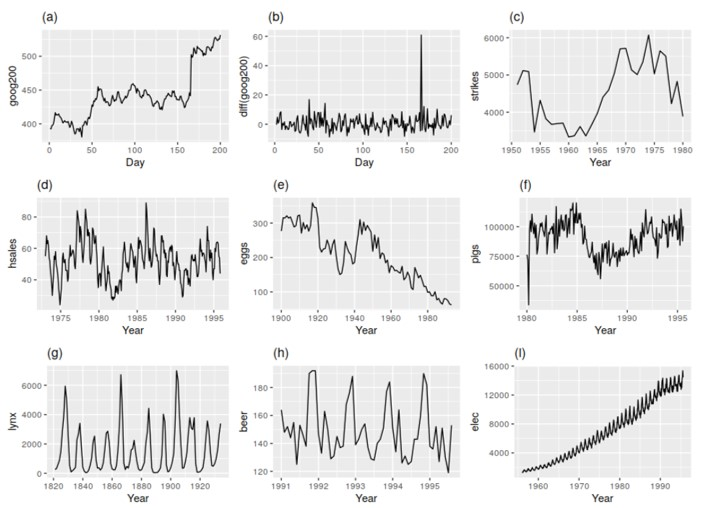
\includegraphics[width=0.9\textwidth]{Imagen1.JPG}
\end{center}
\end{figure}



\end{frame}


%%%%%%%%%%%%%%%%%%%%%%%%%%%%%%%%%%%%%%%%%%%%%%%%%%%%%%%%%%%%




\begin{frame}
\frametitle{Estacionarias?}


\begin{itemize}
\item La estacionalidad obvia descarta las series \textbf{(d)}, \textbf{(h)} e \textbf{(i)}. 
\item Las tendencias y los niveles cambiantes descartan las series \textbf{(a}), \textbf{(c)}, \textbf{(e)}, \textbf{(f)} e \textbf{(i)}. 
\item La varianza creciente también descarta \textbf{(i)}. 
\item Eso deja solo \highlighton{(b)} y \highlighton{(g)} como series estacionarias.
\end{itemize}

\vspace{4mm}

A primera vista, los ciclos fuertes en la serie (g) pueden parecer no estacionarios. Pero estos ciclos son aperiódicos: A largo plazo, el momento de estos ciclos no es predecible. Por lo tanto, la serie es estacionaria.

\end{frame}


%%%%%%%%%%%%%%%%%%%%%%%%%%%%%%%%%%%%%%%%%%%%%%%%%%%%%%%%%%%%



\begin{frame}
\frametitle{Estacionariedad}


Las transformaciones ayudan a \textbf{estabilizar la varianza}. Para los modelos ARIMA, también se necesita \textbf{estabilizar la media}

\vspace{4mm}

\textbf{Identificar series no estacionarias:}

\begin{itemize}
\item Gráfico de serie de tiempo
\item La ACF de datos estacionarios cae a cero relativamente rápido
\item La ACF de datos no estacionarios decrece lentamente
\item Para los datos no estacionarios el valor de $r_1$ es a menudo grande y positivo
\end{itemize}


\end{frame}


%%%%%%%%%%%%%%%%%%%%%%%%%%%%%%%%%%%%%%%%%%%%%%%%%%%%%%%%%%%%


\subsection{Diferenciación}


\begin{frame}
\frametitle{Diferenciación}


\begin{block}{Definición}
Una serie diferenciada es el cambio entre cada observación en la serie original:

\begin{equation}
y'_t = y_t - y_{t-1} 
\end{equation}
\end{block}


\begin{itemize}
\item La diferenciación ayuda a estabilizar la media
\item La diferenciación tendrá solo $(T-1)$ valores ya que no es posible calcular una diferencia $y'_1$ para la primera observación 
\end{itemize}



\end{frame}


%%%%%%%%%%%%%%%%%%%%%%%%%%%%%%%%%%%%%%%%%%%%%%%%%%%%%%%%%%%%




\begin{frame}[fragile]
\frametitle{Ejemplo: Índice Dow-Jones}


\lstset{language=r,label= ,caption= ,captionpos=b,numbers=none}
\begin{lstlisting}
autoplot(dj)
\end{lstlisting}

\pause

\begin{figure}
\begin{center}
    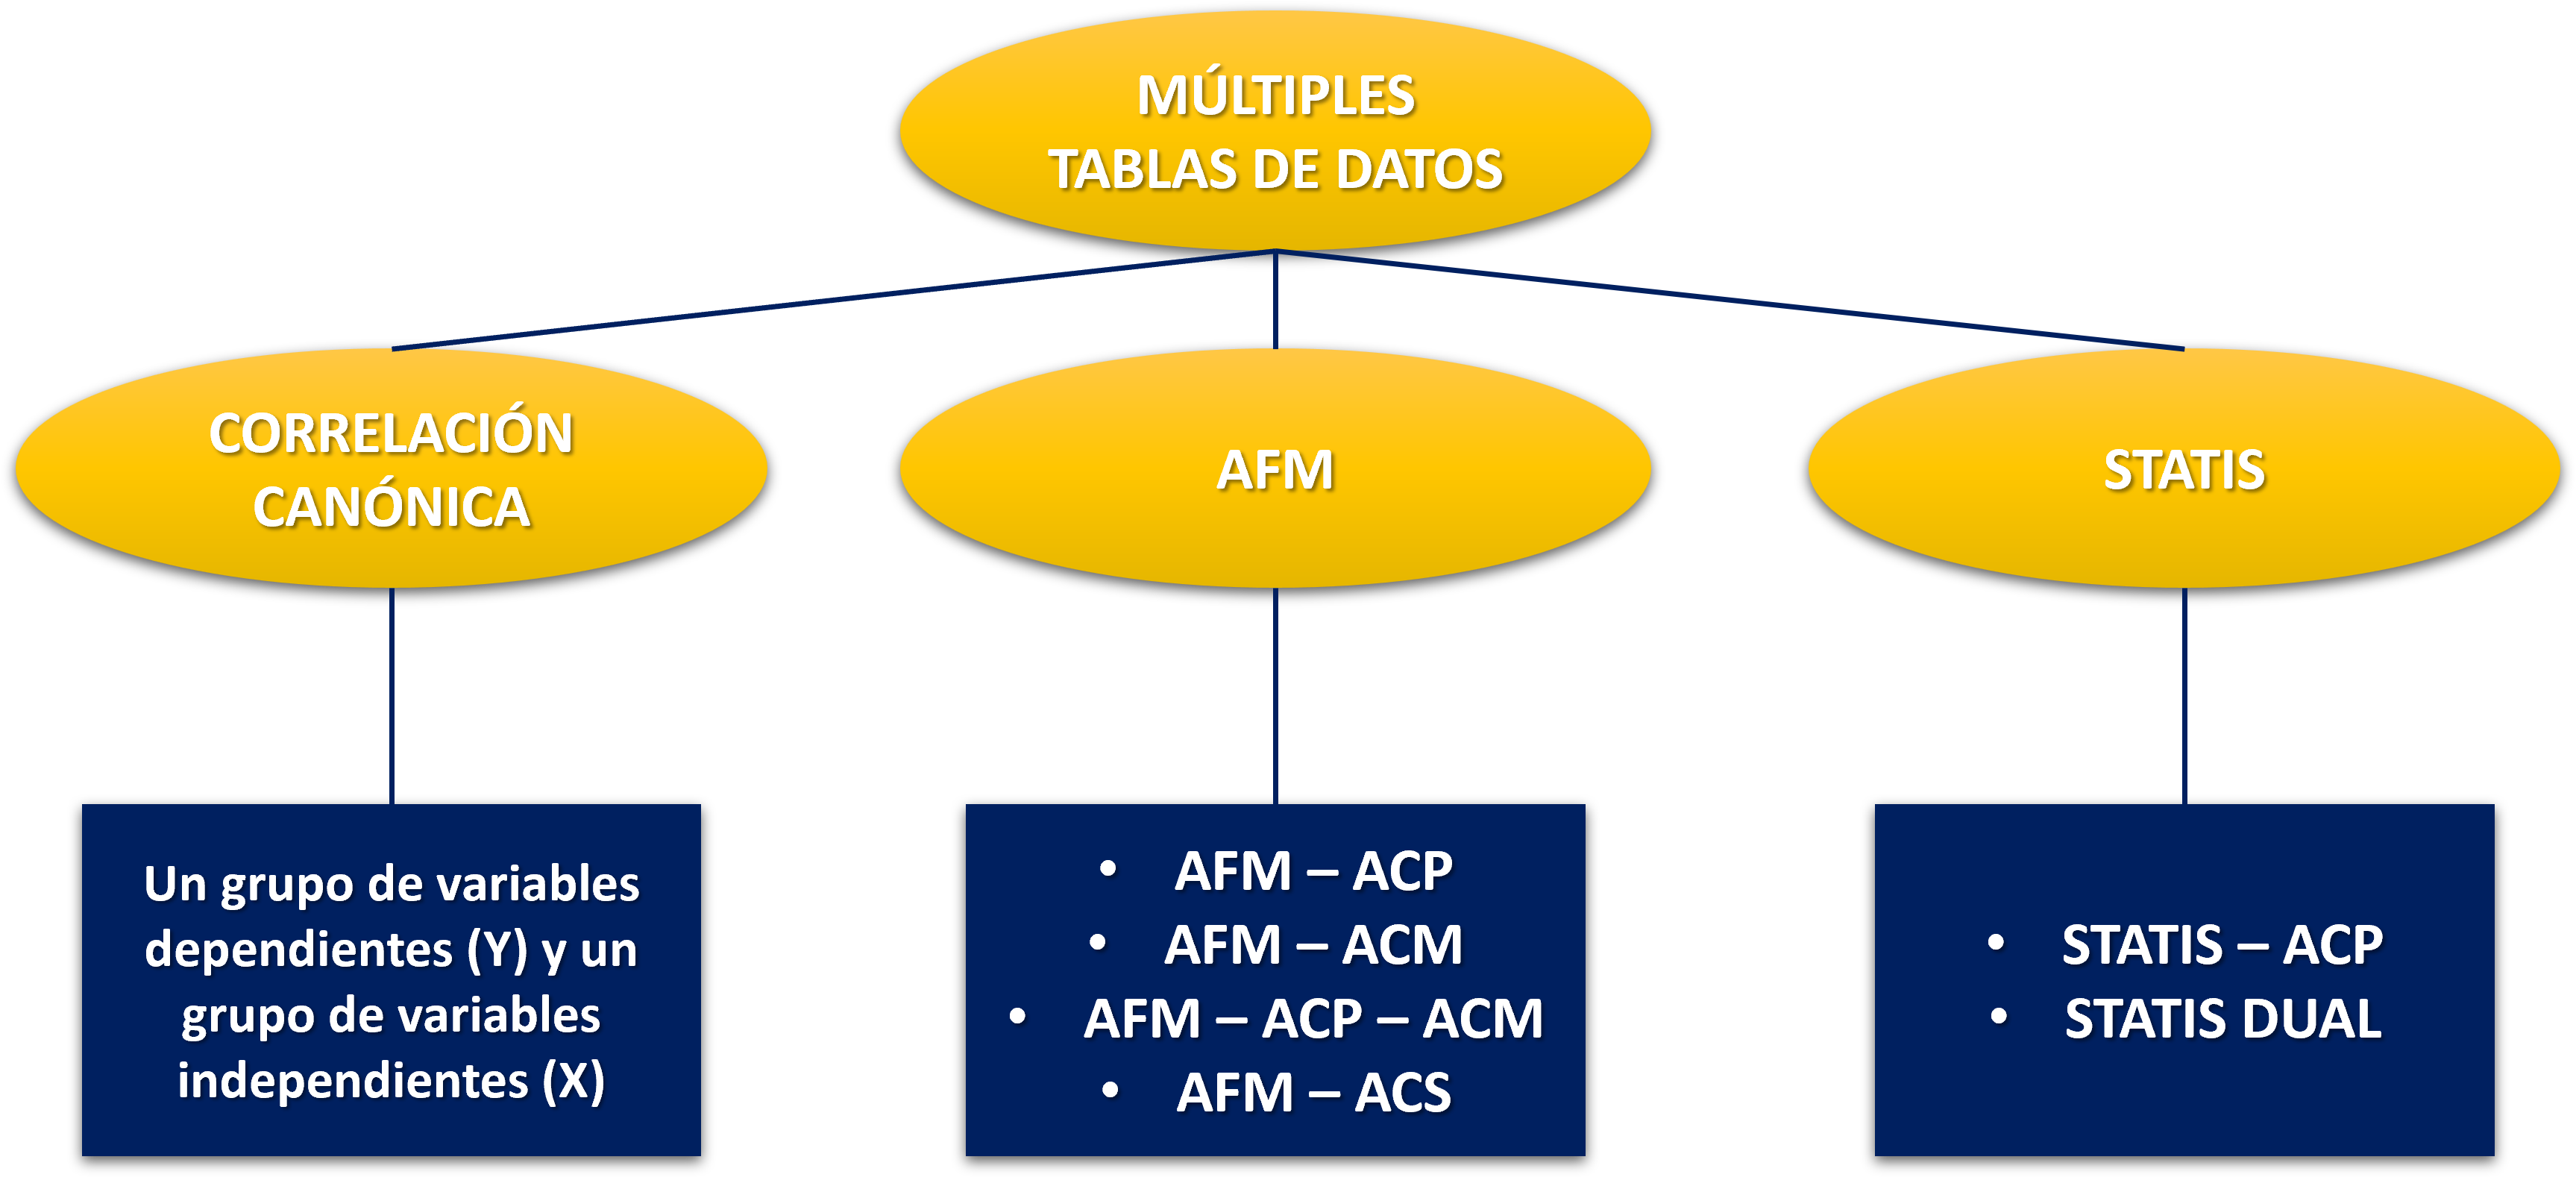
\includegraphics[width=0.9\textwidth]{Imagen2.JPG}
\end{center}
\end{figure}


\end{frame}


%%%%%%%%%%%%%%%%%%%%%%%%%%%%%%%%%%%%%%%%%%%%%%%%%%%%%%%%%%%%





\begin{frame}[fragile]
\frametitle{Ejemplo: Índice Dow-Jones}


\lstset{language=r,label= ,caption= ,captionpos=b,numbers=none}
\begin{lstlisting}
ggAcf(dj)
\end{lstlisting}

\pause

\begin{figure}
\begin{center}
    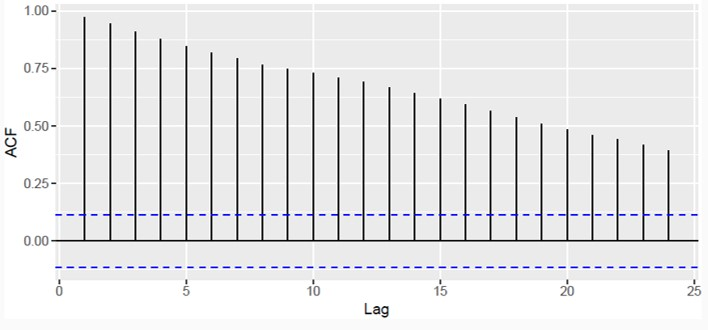
\includegraphics[width=0.9\textwidth]{Imagen3.JPG}
\end{center}
\end{figure}


\end{frame}


%%%%%%%%%%%%%%%%%%%%%%%%%%%%%%%%%%%%%%%%%%%%%%%%%%%%%%%%%%%%







\begin{frame}[fragile]
\frametitle{Ejemplo: Índice Dow-Jones}


\lstset{language=r,label= ,caption= ,captionpos=b,numbers=none}
\begin{lstlisting}
diff(dj)
\end{lstlisting}

\pause

\begin{figure}
\begin{center}
    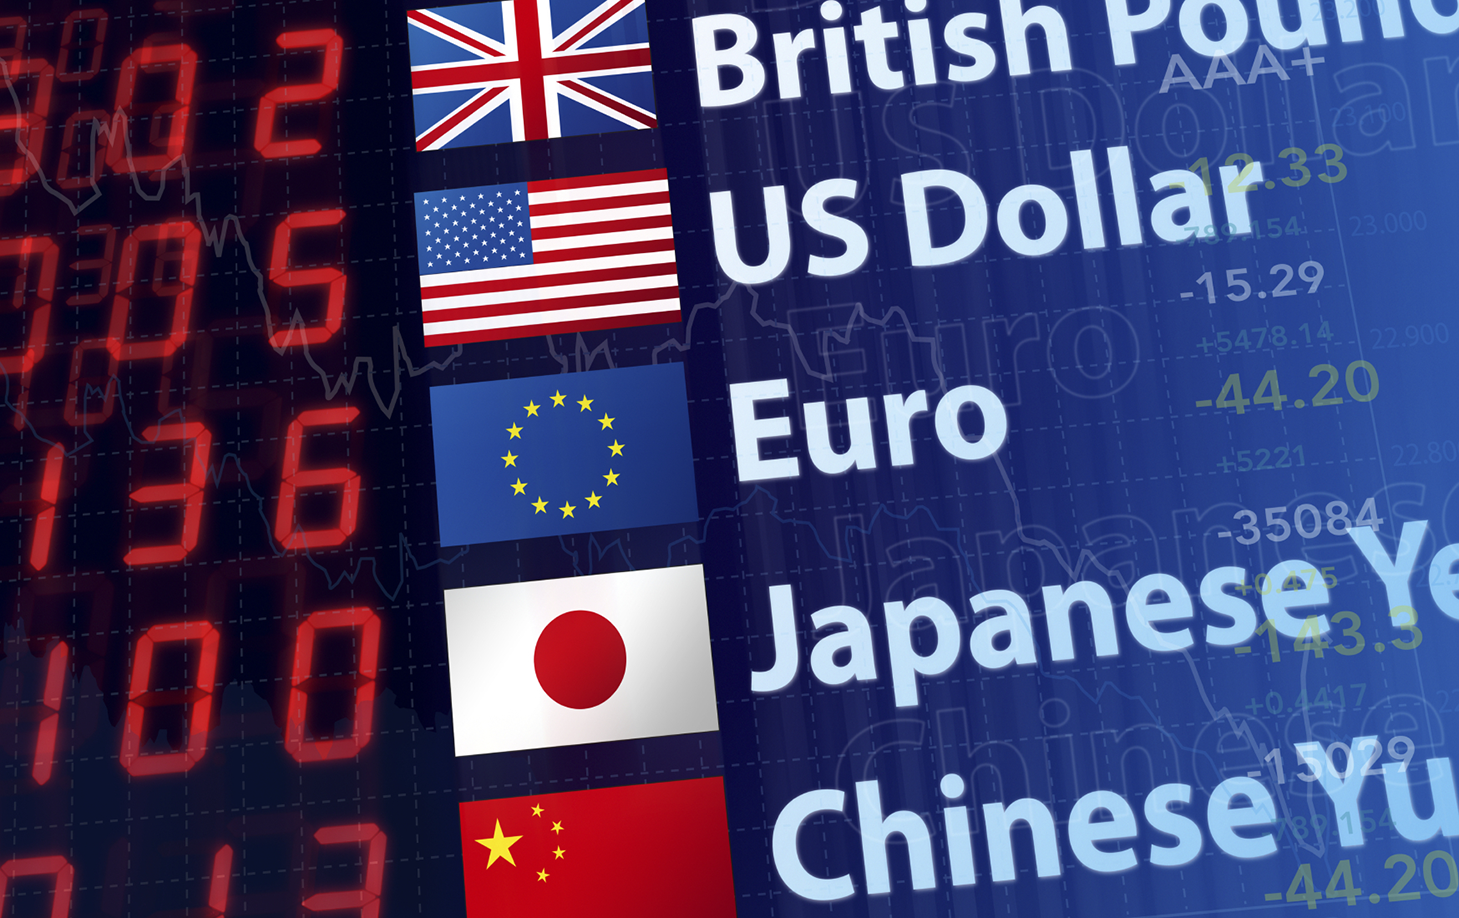
\includegraphics[width=0.9\textwidth]{Imagen4.JPG}
\end{center}
\end{figure}


\end{frame}


%%%%%%%%%%%%%%%%%%%%%%%%%%%%%%%%%%%%%%%%%%%%%%%%%%%%%%%%%%%%




\begin{frame}[fragile]
\frametitle{Ejemplo: Índice Dow-Jones}


\lstset{language=r,label= ,caption= ,captionpos=b,numbers=none}
\begin{lstlisting}
ggAcf(diff(dj))
\end{lstlisting}

\pause

\begin{figure}
\begin{center}
    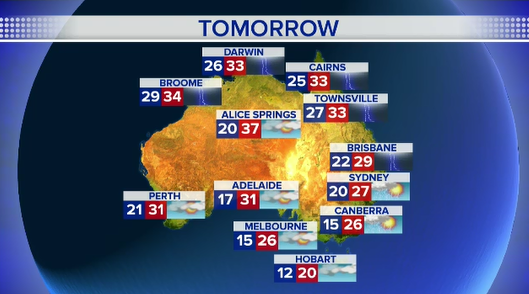
\includegraphics[width=0.9\textwidth]{Imagen5.JPG}
\end{center}
\end{figure}


\end{frame}


%%%%%%%%%%%%%%%%%%%%%%%%%%%%%%%%%%%%%%%%%%%%%%%%%%%%%%%%%%%%



\begin{frame}[fragile]
\frametitle{Ejercicio}


Evalúe la estacionariedad para la serie goog200. Posteriormente realice la diferenciación y evalúe la estacionariedad sobre los cambios en la serie goog200.

\vspace{4mm}

Realice la prueba de Ljung-Box para cada series (Original y diferenciada) para determinar si existe correlación entre las observaciones. Utilice lag = 10.


\begin{center}
\highlighton{¿Que puede concluir?}
\end{center}

\pause

\lstset{language=r,label= ,caption= ,captionpos=b,numbers=none}
\begin{lstlisting}
Box.test(goog200, lag=10, type="Ljung-Box")
Box.test(diff(goog200), lag=10, type="Ljung-Box")
\end{lstlisting}




\end{frame}


%%%%%%%%%%%%%%%%%%%%%%%%%%%%%%%%%%%%%%%%%%%%%%%%%%%%%%%%%%%%



%%%%%%%%%%%%%%%%%%%%%%%%%%%%%%%%%%%%%%%%%%%%%%%%%%%%%%%%%%%%

\subsection{Diferenciación de segundo orden}

\begin{frame}[fragile]
\frametitle{Diferenciación de segundo orden}


Ocasionalmente, los datos diferenciados no parecerán estacionarios y puede ser necesario diferenciar los datos por segunda vez para obtener una serie estacionaria:


\begin{eqnarray}
y''_t & = & y'_t - y'_{t-1} \\
      & = & (y_t - y_{t-1}) - (y_{t-1} - y_{t-2}) \\
      & = & y_t - 2y_{t-1} +  y_{t-2}
\end{eqnarray}

\vspace{4mm}

\begin{itemize}
\item En este caso, $y''_t$ tendrá $T-2$ valores
\item En la práctica, casi nunca es necesario ir más allá de las diferencias de segundo orden.
\end{itemize}



\end{frame}


%%%%%%%%%%%%%%%%%%%%%%%%%%%%%%%%%%%%%%%%%%%%%%%%%%%%%%%%%%%%



\subsection{Diferenciación Estacional}

\begin{frame}[fragile]
\frametitle{Diferenciación Estacional}


Una diferencia estacional es la diferencia entre una observación y la observación previa de la misma estación. Entonces

\begin{eqnarray}
y'_t = y_t - y_{t-m}
\end{eqnarray}

\vspace{4mm}


\begin{itemize}
\item m = número de estaciones
\item m = 12 (Para datos mensuales)
\item m = 4 (Para datos trimestrales)
\end{itemize}



\end{frame}


%%%%%%%%%%%%%%%%%%%%%%%%%%%%%%%%%%%%%%%%%%%%%%%%%%%%%%%%%%%%




\begin{frame}[fragile]
\frametitle{Ejemplo}


Analicemos la serie a10 (Venta de medicamentos antidiabéticos). Es Estacionaria la serie?



\lstset{language=r,label= ,caption= ,captionpos=b,numbers=none}
\begin{lstlisting}
autoplot(a10)
\end{lstlisting}

\pause


\begin{figure}
\begin{center}
    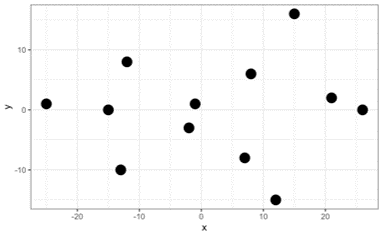
\includegraphics[width=0.7\textwidth]{Imagen6.JPG}
\end{center}
\end{figure}



\end{frame}


%%%%%%%%%%%%%%%%%%%%%%%%%%%%%%%%%%%%%%%%%%%%%%%%%%%%%%%%%%%%





\begin{frame}[fragile]
\frametitle{Ejemplo}


\lstset{language=r,label= ,caption= ,captionpos=b,numbers=none}
\begin{lstlisting}
cbind("Sales ($million)" = a10,
      "Monthly log sales" = log(a10),
      "Annual change in log sales" = diff(log(a10),12)) %>%
  autoplot(facets=TRUE) +
    xlab("Year") + ylab("") +
    ggtitle("Antidiabetic drug sales")
\end{lstlisting}

\pause

\vspace{4mm}

\begin{itemize}
\item Para distinguir las diferencias estacionales de las diferencias ordinarias, a veces nos referimos a las diferencias ordinarias como \textcolor{teal}{\textbf{``primeras diferencias''}}, lo que significa diferencias en el rezago 1.

\item La transformación y la diferenciación harán que la serie parezca relativamente estacionaria.
\end{itemize}




\end{frame}


%%%%%%%%%%%%%%%%%%%%%%%%%%%%%%%%%%%%%%%%%%%%%%%%%%%%%%%%%%%%



\begin{frame}[fragile]
\frametitle{Ejemplo}



\begin{figure}
\begin{center}
    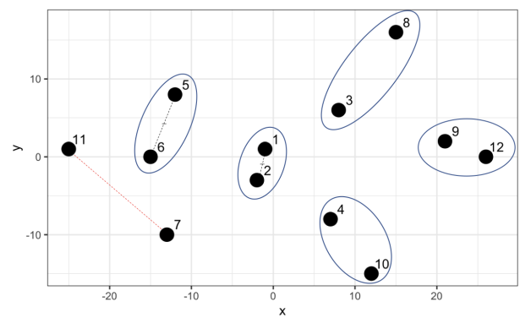
\includegraphics[width=0.6\textwidth]{Imagen7.JPG}
\end{center}
\end{figure}



\end{frame}


%%%%%%%%%%%%%%%%%%%%%%%%%%%%%%%%%%%%%%%%%%%%%%%%%%%%%%%%%%%%



\begin{frame}[fragile]
\frametitle{Ejercicio}

A veces es necesario tomar una diferencia estacional y una primera diferencia para obtener datos estacionarios.

\vspace{4mm}

De tal manera, diferencie estacionalmente la serie usmelec (generación de electricidad). Es decir, como el ejemplo anterior realice la transformación, diferencia estacional y posteriormente diferencie la diferenciación estacional.



\end{frame}


%%%%%%%%%%%%%%%%%%%%%%%%%%%%%%%%%%%%%%%%%%%%%%%%%%%%%%%%%%%%




\begin{frame}[fragile]
\frametitle{Ejercicio}



\begin{figure}
\begin{center}
    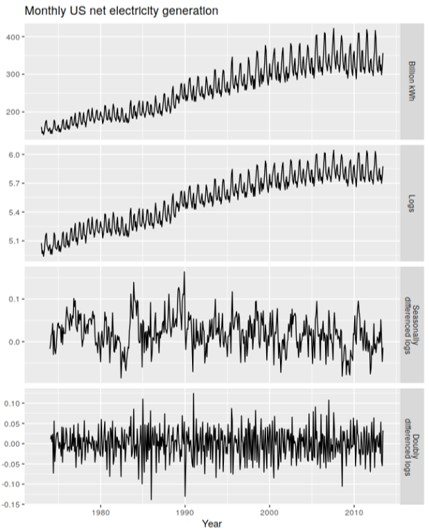
\includegraphics[width=0.5\textwidth]{Imagen8.JPG}
\end{center}
\end{figure}



\end{frame}




%%%%%%%%%%%%%%%%%%%%%%%%%%%%%%%%%%%%%%%%%%%%%%%%%%%%%%%%%%%%

\begin{frame}[fragile]
\frametitle{Ejercicio}

{\small
\begin{itemize}
\item Hay un grado de subjetividad en la selección de las diferencias a aplicar. 
\item Los datos diferenciados estacionalmente en \textcolor{red}{a10} no muestran un comportamiento sustancialmente diferente de los datos diferenciados estacionalmente en \textcolor{blue}{usmelec}. 
\item En el último caso, podríamos haber decidido detenernos con los datos diferenciados estacionalmente, y no haber hecho una ronda adicional de diferenciación. 
\item En el primer caso, podríamos haber decidido que los datos no eran lo suficientemente estacionarios y haber tomado una ronda adicional de diferenciación.
 
\vspace{3mm}

\highlighton{Siempre hay que tomar algunas decisiones en el proceso de modelado, y diferentes analistas pueden tomar diferentes decisiones.}
\end{itemize}
}


\end{frame}


%%%%%%%%%%%%%%%%%%%%%%%%%%%%%%%%%%%%%%%%%%%%%%%%%%%%%%%%%%%%




\begin{frame}[fragile]
\frametitle{Ejercicio}

\textbf{Código usmelec.}

\lstset{language=r,label= ,caption= ,captionpos=b,numbers=none}
\begin{lstlisting}
cbind("Billion kWh" = usmelec,
      "Logs" = log(usmelec),
      "Seasonally\n differenced logs" =
        diff(log(usmelec),12),
      "Doubly\n differenced logs" =
        diff(diff(log(usmelec),12),1)) %>%
  autoplot(facets=TRUE) +
    xlab("Year") + ylab("") +
    ggtitle("Monthly US net electricity generation")
\end{lstlisting}


\end{frame}


%%%%%%%%%%%%%%%%%%%%%%%%%%%%%%%%%%%%%%%%%%%%%%%%%%%%%%%%%%%%





\begin{frame}[fragile]
\frametitle{Diferenciación Estacional}

Cuando se aplican tanto las diferencias estacionales como las primeras, no importa qué se haga primero: el resultado será el mismo. 

\vspace{3mm}

{\small
\begin{itemize}
\item Sin embargo, si los datos tienen un \textcolor{teal}{patrón estacional} fuerte, \textbf{\textit{se recomienda}} hacer primero la diferenciación estacional, porque las series resultantes a veces serán estacionarias y no habrá necesidad de una primera diferencia adicional. 

\item Si la primera diferenciación se realiza primero, aún habrá estacionalidad presente.
\end{itemize}
}

\vspace{3mm}
\pause

{\small
\begin{block}{Ojo con las interpretaciones de las diferenciaciones}
Las primeras diferencias son el cambio entre una observación y la siguiente. Las diferencias estacionales son el cambio entre un año y el siguiente. Es poco probable que otros retrasos tengan mucho sentido interpretable y deben evitarse.
\end{block}
}
\end{frame}


%%%%%%%%%%%%%%%%%%%%%%%%%%%%%%%%%%%%%%%%%%%%%%%%%%%%%%%%%%%%



\subsection{Test de raíz unitaria}


\begin{frame}[fragile]
\frametitle{Test de raíz unitaria}

\textcolor{teal}{Estas son pruebas de hipótesis estadísticas de estacionariedad diseñadas para determinar si se requiere diferenciación.}

\vspace{3mm}

Hay disponibles varias pruebas de raíz unitaria, que se basan en supuestos diferentes y pueden dar lugar a respuestas conflictivas.


\begin{enumerate}
\item Test aumentado de Dickey Fuller: Hipótesis nula es que los datos son no estacionarios y no estacionales.

\item Test Kwiatkowski-Phillips-Schmidt-Shin (KPSS): Hipótesis nula es que los datos son estacionarios y no estacionales.

\item Otros test disponibles para datos estacionales.
\end{enumerate}

\end{frame}


%%%%%%%%%%%%%%%%%%%%%%%%%%%%%%%%%%%%%%%%%%%%%%%%%%%%%%%%%%%%




\begin{frame}[fragile]
\frametitle{Test de raíz unitaria}

\textbf{Test KPSS}

\lstset{language=r,label= ,caption= ,captionpos=b,numbers=none}
\begin{lstlisting}
library(urca)
summary(ur.kpss(goog))
\end{lstlisting}

\pause

{\scriptsize
\begin{verbatim}
####################### 
# KPSS Unit Root Test # 
####################### 

Test is of type: mu with 7 lags. 

Value of test-statistic is: 10.7223 

Critical value for a significance level of: 
                10pct  5pct 2.5pct  1pct
critical values 0.347 0.463  0.574 0.739
\end{verbatim}
}

\pause

{\small
\begin{block}{Interpretación}
El estadístico de prueba \textbf{\highlighton{(10.72)}} es mucho mayor que el valor crítico del 1\% \highlighton{(0.739)}, lo que indica que la hipótesis nula es rechazada. Es decir, \textcolor{teal}{los datos no son estacionarios}. Podemos diferenciar los datos y aplicar la prueba nuevamente.
\end{block}
}


\end{frame}


%%%%%%%%%%%%%%%%%%%%%%%%%%%%%%%%%%%%%%%%%%%%%%%%%%%%%%%%%%%%


\begin{frame}[fragile]
\frametitle{Test de raíz unitaria}

\textbf{Test aumentado de Dickey Fuller}

\lstset{language=r,label= ,caption= ,captionpos=b,numbers=none}
\begin{lstlisting}
library(tseries)
adf.test(goog)
\end{lstlisting}

\pause

{\scriptsize
\begin{verbatim}
	Augmented Dickey-Fuller Test

data:  goog
Dickey-Fuller = -2.5417, Lag order = 9, p-value = 0.349
alternative hypothesis: stationary
\end{verbatim}
}

\pause

{\small
\begin{block}{Interpretación}
No rechaza la hipótesis nula. Por lo tanto los datos de goog son \textcolor{teal}{no estacionarios}
\end{block}
}


\end{frame}


%%%%%%%%%%%%%%%%%%%%%%%%%%%%%%%%%%%%%%%%%%%%%%%%%%%%%%%%%%%%







\begin{frame}[fragile]
\frametitle{Test de raíz unitaria}


\lstset{language=r,label= ,caption= ,captionpos=b,numbers=none}
\begin{lstlisting}
library(urca)
summary(ur.kpss(diff(goog)))
\end{lstlisting}

\pause

{\scriptsize
\begin{verbatim}
####################### 
# KPSS Unit Root Test # 
####################### 

Test is of type: mu with 7 lags. 

Value of test-statistic is: 0.0324 

Critical value for a significance level of: 
                10pct  5pct 2.5pct  1pct
critical values 0.347 0.463  0.574 0.739
\end{verbatim}
}

\pause

{\small
\begin{block}{Interpretación}
Esta vez, el estadístico de prueba \textbf{\highlighton{(0.0324)}} es pequeño y está dentro del rango que esperaríamos para los datos estacionarios. Entonces podemos concluir que \textcolor{teal}{los datos diferenciados son estacionarios.}
\end{block}
}


\end{frame}


%%%%%%%%%%%%%%%%%%%%%%%%%%%%%%%%%%%%%%%%%%%%%%%%%%%%%%%%%%%%





\begin{frame}[fragile]
\frametitle{Test de raíz unitaria}


La función lleva a cabo este proceso de usar una secuencia de pruebas KPSS para determinar el número apropiado de primeras diferencias

\lstset{language=r,label= ,caption= ,captionpos=b,numbers=none}
\begin{lstlisting}
ndiffs(goog)
\end{lstlisting}

\pause

{\scriptsize
\begin{verbatim}
[1] 1
\end{verbatim}
}

Como vimos en las pruebas de KPSS anteriores, se requiere una diferencia para que los datos de goog sean estacionarios.


\pause
{\small
\begin{block}{}
Una función similar para determinar si se requiere diferenciación estacional es la \highlighton{nsdiffs()} para determinar el número apropiado de diferencias estacionales requeridas. 

\vspace{4mm}
Descomposición STL: $ y_t = T_t + S_t + R_t$\\
Fuerza estacional: $F_s = max(0, 1- \frac{Var(R_t)}{Var(S_t+R_t)})$\\
Si $F_s > 0.64$ hacer una diferenciación estacional.
\end{block}
}

\end{frame}


%%%%%%%%%%%%%%%%%%%%%%%%%%%%%%%%%%%%%%%%%%%%%%%%%%%%%%%%%%%%





\begin{frame}[fragile]
\frametitle{Test de raíz unitaria}


Podemos aplicar \textbf{nsdiffs()} a los datos de electricidad mensuales registrados en los EE. UU.


\lstset{language=r,label= ,caption= ,captionpos=b,numbers=none}
\begin{lstlisting}
usmelec %>% log() %>% nsdiffs()
\end{lstlisting}


{\scriptsize
\begin{verbatim}
[1] 1
\end{verbatim}
}


\lstset{language=r,label= ,caption= ,captionpos=b,numbers=none}
\begin{lstlisting}
usmelec %>% log() %>% diff(lag=12) %>% ndiffs()
\end{lstlisting}


{\scriptsize
\begin{verbatim}
[1] 1
\end{verbatim}
}


\begin{itemize}
\item Debido a que nsdiffs( )devuelve 1 (lo que indica que se requiere una diferencia estacional), aplicamos la función ndiffs() a los datos diferenciados estacionalmente. 

\item Estas funciones sugieren que deberíamos hacer una diferencia estacional y una primera diferencia.
\end{itemize}




\end{frame}


%%%%%%%%%%%%%%%%%%%%%%%%%%%%%%%%%%%%%%%%%%%%%%%%%%%%%%%%%%%%




\begin{frame}[fragile]
\frametitle{Test de raíz unitaria}

\textbf{Test aumentado de Dickey Fuller}

\lstset{language=r,label= ,caption= ,captionpos=b,numbers=none}
\begin{lstlisting}
library(tseries)
adf.test(diff(goog))
\end{lstlisting}

\pause

{\scriptsize
\begin{verbatim}

	Augmented Dickey-Fuller Test

data:  diff(goog)
Dickey-Fuller = -11.157, Lag order = 9, p-value = 0.01
alternative hypothesis: stationary

\end{verbatim}
}

\pause

{\small
\begin{block}{Interpretación}
Rechaza la hipótesis nula. Por lo tanto los datos de goog son \textcolor{teal}{estacionarios}
\end{block}
}


\end{frame}


%%%%%%%%%%%%%%%%%%%%%%%%%%%%%%%%%%%%%%%%%%%%%%%%%%%%%%%%%%%%



%%%%%%%%%%%%%%%%%%%%%%%%%%%%%%%%%%%%%%%%%%%%%%%%%%%%%%%%%%%%


\section{Modelos autorregresivos}



\begin{frame}[fragile]
\frametitle{Modelos Autorregresivos}


En un modelo de regresión múltiple, pronosticamos la variable de interés utilizando una combinación lineal de predictores. 

\vspace{4mm}

En un modelo autorregresivo, pronosticamos la variable de interés utilizando una \textcolor{blue}{combinación lineal de valores pasados de la variable}. El término auto regresión indica que es una regresión de la variable contra sí misma.

\vspace{4mm}

\begin{block}{Modelo autorregresivo de  \textbf{orden p}}
\begin{equation}
 y_{t}  =  c  +  \phi_{1}y_{t - 1}  +  \phi_{2}y_{t - 2}  +  ...  +  \phi_{p}y_{t - p}  + \varepsilon_{t}
\end{equation}

dónde $\varepsilon_t$ es ruido blanco.

\end{block}

\begin{center}
\highlighton{\textbf{Nos referimos como un AR(p) a un modelo autorregresivo de orden p.}}
\end{center}


\end{frame}


%%%%%%%%%%%%%%%%%%%%%%%%%%%%%%%%%%%%%%%%%%%%%%%%%%%%%%%%%%%%



\begin{frame}[fragile]
\frametitle{Modelos Autorregresivos}


Los modelos autorregresivos son notablemente flexibles para manejar una amplia gama de patrones de series temporales diferentes.

\vspace{4mm}


\begin{figure}
\begin{center}
    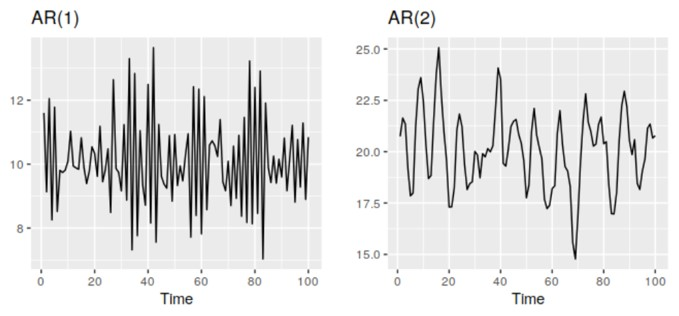
\includegraphics[width=0.6\textwidth]{Imagen9.JPG}
\end{center}
\end{figure}


Cambiar los parámetros $\phi_1, ..., \phi_p$ da como resultado diferentes patrones de series de tiempo. La varianza del término de error $\varepsilon_t$ sólo cambiara la escala de la serie, no los patrones.

\end{frame}


%%%%%%%%%%%%%%%%%%%%%%%%%%%%%%%%%%%%%%%%%%%%%%%%%%%%%%%%%%%%





\begin{frame}[fragile]
\frametitle{Modelos Autorregresivos}


Para un modelo \textbf{AR(1)}:
\vspace{4mm}


\begin{block}{}
\begin{equation}
y_{t}  =  c  +  \phi_{1}y_{t - 1} + \varepsilon_{t}
\end{equation}
\end{block}


\begin{itemize}
\item Cuando $\phi_1 = 0$, $y_t$ es equivalente al ruido blanco.
\item Cuando $\phi_1 = 1$ y $C = 0$, $y_t$ es equivalente a una caminata aleatoria.
\item Cuando $\phi_1 = 1$ y $C \neq 0$, $y_t$ es equivalente a una caminata aleatoria con deriva.
\item Cuando $\phi_1 < 0$, $y_t$ tiende a oscilar alrededor de la media.
\end{itemize}

\end{frame}


%%%%%%%%%%%%%%%%%%%%%%%%%%%%%%%%%%%%%%%%%%%%%%%%%%%%%%%%%%%%




\begin{frame}[fragile]
\frametitle{Modelos Autorregresivos}


Normalmente restringimos los modelos autorregresivos a datos estacionarios, en cuyo caso se requieren algunas restricciones en los valores de los parámetros.

\vspace{4mm}

\begin{itemize}
\item Para un modelo AR(1): $-1 < \phi_1 < 1$
\item Para un modelo AR(2): $-1 < \phi_2 < 1$, $\phi_1 + \phi_2 < 1$, $\phi_2 - \phi_1 < 1$
\item Para un modelo AR(3): Las condiciones son más complicadas. El software se encarga de estas restricciones al estimar el modelo.
\end{itemize}

\end{frame}


%%%%%%%%%%%%%%%%%%%%%%%%%%%%%%%%%%%%%%%%%%%%%%%%%%%%%%%%%%%%


\section{Modelos de media móvil}


\begin{frame}[fragile]
\frametitle{Modelo de media móvil}


En lugar de usar valores pasados de la variable de pronóstico en una regresión, un modelo de promedio móvil usa errores de pronóstico pasados en un modelo similar a la regresión.


\begin{block}{Modelo de medias móviles de \textbf{orden q}}
\begin{equation}
 y_{t}  =  c +  \varepsilon_t + \theta_{1}\varepsilon_{t - 1}  +  \theta_{2}\varepsilon_{t - 2}  +  \cdots  + \theta_{q}\varepsilon_{t - q}
\end{equation}

dónde $\varepsilon_t$ es ruido blanco.
\end{block}

Por supuesto, no observamos los valores de $\varepsilon_t$ por lo que no es realmente una regresión en el sentido habitual.


\begin{center}
\highlighton{\textbf{Nos referimos como un MA(q) a un modelo de medias móviles de orden q.}}
\end{center}

\end{frame}


%%%%%%%%%%%%%%%%%%%%%%%%%%%%%%%%%%%%%%%%%%%%%%%%%%%%%%%%%%%%



\begin{frame}[fragile]
\frametitle{Modelo de media móvil}

{\small
Cada valor de $y_t$ puede considerarse como un promedio móvil ponderado de los últimos errores de pronóstico. Sin embargo, los modelos de promedio móvil no deben confundirse con el suavizado del promedio móvil.

\vspace{4mm}

Se usa un modelo de promedio móvil para pronosticar valores futuros, mientras que el suavizado de promedio móvil se usa para estimar el ciclo de tendencia de valores pasados.
}
\begin{figure}
\begin{center}
    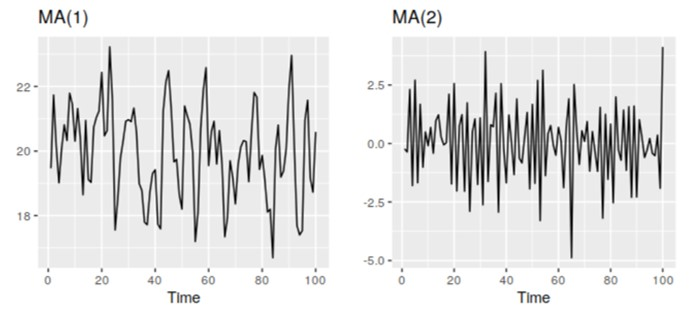
\includegraphics[width=0.5\textwidth]{Imagen10.JPG}
\end{center}
\end{figure}

\pause
{\small
Cambiar los parámetros $\theta_1, ..., \theta_q$ da como resultado diferentes patrones de series de tiempo. La varianza del término de error $\varepsilon_t$ sólo cambiara la escala de la serie, no los patrones.
}
\end{frame}


%%%%%%%%%%%%%%%%%%%%%%%%%%%%%%%%%%%%%%%%%%%%%%%%%%%%%%%%%%%%


\begin{frame}[fragile]
\frametitle{Modelos MA($\infty$)}


Es posible escribir cualquier modelo estacionario AR(p) como un modelo MA($\infty$). Por ejemplo, usando la sustitución repetida, podemos demostrar esto para un modelo AR(1):


\begin{align*}
y_t &= \phi_1y_{t-1} + \varepsilon_t\\
&= \phi_1(\phi_1y_{t-2} + \varepsilon_{t-1}) + \varepsilon_t\\
&= \phi_1^2y_{t-2} + \phi_1 \varepsilon_{t-1} + \varepsilon_t\\
&= \phi_1^3y_{t-3} + \phi_1^2\varepsilon_{t-2} + \phi_1 \varepsilon_{t-1} + \varepsilon_t\\
& ...
\end{align*}

\begin{itemize}
\item Previsto $-1 < \phi_1 < 1$:\\
\begin{equation}
y_t = \varepsilon_t + \phi_1 \varepsilon_{t-1} + \phi_1^2 \varepsilon_{t-2} + \phi_1^3 \varepsilon_{t-3} + ...
\end{equation}

\end{itemize}

\end{frame}


%%%%%%%%%%%%%%%%%%%%%%%%%%%%%%%%%%%%%%%%%%%%%%%%%%%%%%%%%%%%



\begin{frame}[fragile]
\frametitle{Invertibilidad}


\begin{itemize}
\item Cualquier proceso $MA(q)$ puede escribirse como un proceso $AR(\infty)$ si imponemos algunas restricciones en los parámetros $MA$

\item Entonces el modelo $MA$ es llamado ``Invertible''

\item Los modelos invertibles tienen algunas propiedades matemáticas que los hace más fácil de usar en la práctica.

\end{itemize}

\end{frame}


%%%%%%%%%%%%%%%%%%%%%%%%%%%%%%%%%%%%%%%%%%%%%%%%%%%%%%%%%%%%


\begin{frame}[fragile]
\frametitle{Invertibilidad}


Considere un proceso $MA(1)$, $y_t = \varepsilon_t + \theta_1 \varepsilon_{t-1}$. En su representación $AR(\infty)$, el error más reciente puede ser escrito como una función lineal de las observaciones actuales y pasadas.


\begin{equation}
\varepsilon_t = \sum_{j=0}^{\infty} (-\theta)^j y_{t-j}
\end{equation}


\begin{itemize}
\item Requerimos que $|\theta| < 1$, por lo que las observaciones más recientes tienen mayor peso que las observaciones del pasado más lejano. Por lo tanto el proceso es invertible cuando $|\theta| < 1$

\end{itemize}

\end{frame}


%%%%%%%%%%%%%%%%%%%%%%%%%%%%%%%%%%%%%%%%%%%%%%%%%%%%%%%%%%%%



\begin{frame}[fragile]
\frametitle{Invertibilidad}


\begin{block}{Condición general de invertibilidad}
Las raíces complejas de $1+\theta_1 z + \theta_2 z^2 + \dots + \theta_qz^q$ se encuentran fuera del circulo unitario en el plano complejo.
\end{block}

\vspace{4mm}

Las restricciones de invertibilidad para otros modelos son similares a las restricciones de estacionariedad.

\vspace{3mm}

\begin{itemize}
\item Para un modelo MA(1): $-1 < \theta_1 < 1$
\item Para un modelo MA(2): $-1<\theta_2<1\qquad \theta_2+\theta_1 >-1 \qquad \theta_1 -\theta_2 < 1$.
\item Para un modelo MA(3): Las condiciones son más complicadas. El software se encarga de estas restricciones al estimar el modelo.
\end{itemize}

\end{frame}


%%%%%%%%%%%%%%%%%%%%%%%%%%%%%%%%%%%%%%%%%%%%%%%%%%%%%%%%%%%%


\section{Modelos ARIMA}



\begin{frame}[fragile]
\frametitle{ARIMA}


\small Si combinamos la diferenciación con autorregresión y un modelo de media móvil, obtenemos un modelo ARIMA no estacional. ARIMA es un acrónimo de AutoRegressive Integrated Moving Average (en este contexto, ``integración'' es lo contrario de la diferenciación).

\begin{block}{ARMA:}
\begin{align*}
y_{t}  &=  c  +  \phi_{1}y_{t - 1}  +  \cdots  +  \phi_{p}y_{t - p} \\
& \hspace*{2.4cm}\text{} + \theta_{1}\varepsilon_{t - 1} +  \cdots  + \theta_{q}\varepsilon_{t - q} +  \varepsilon_{t}
\end{align*}
\end{block}

\vspace{4mm}


\begin{itemize}
\item Los predictores incluyen valores rezagados de $y_t$ y errores rezagados.
\item Las condiciones sobre los coeficientes aseguran la estacionariedad.
\item Las condiciones sobre los coeficientes aseguran la invertibilidad.
\end{itemize}

\end{frame}


%%%%%%%%%%%%%%%%%%%%%%%%%%%%%%%%%%%%%%%%%%%%%%%%%%%%%%%%%%%%



\begin{frame}[fragile]
\frametitle{ARIMA}


\textcolor{teal}{\textbf{AutoRegressive Integrated Moving Average (ARIMA)}}

\begin{block}{ARIMA($p, d, q$)}
\begin{tabular}{rl}
AR:& $p =$  orden de la parte autorrgresiva\\
I: & $d =$  grado de la primera diferenciación\\
MA:& $q =$  orden de la parte de medias móviles
\end{tabular}
\end{block}

\vspace{4mm}


\begin{itemize}
\item Modelo ruido blanco:  ARIMA(0,0,0)
\item Caminata aleatoria:  ARIMA(0,1,0) sin constante
\item Caminata aleatoria con deriva:  ARIMA(0,1,0) con constante
\item AR($p$): ARIMA($p$,0,0)
\item MA($q$): ARIMA(0,0,$q$)
\end{itemize}

\end{frame}


%%%%%%%%%%%%%%%%%%%%%%%%%%%%%%%%%%%%%%%%%%%%%%%%%%%%%%%%%%%%



\begin{frame}[fragile]
\frametitle{Ejemplo}

La serie $(uschange[,``Consumption''])$ muestra los cambios porcentuales trimestrales en el gasto de consumo de los Estados Unidos. Aunque es una serie trimestral, no parece haber un patrón estacional, por lo que ajustaremos un \textbf{modelo ARIMA no estacional}.



\lstset{language=r,label= ,caption= ,captionpos=b,numbers=none}
\begin{lstlisting}
autoplot(uschange[,"Consumption"]) +
  xlab("Year") + ylab("Quarterly percentage change")
\end{lstlisting}

\pause


\begin{figure}
\begin{center}
    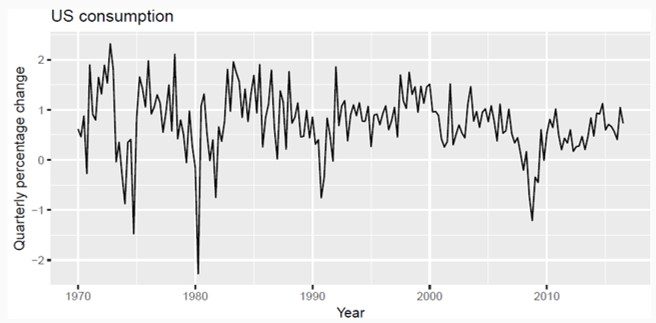
\includegraphics[width=0.7\textwidth]{Imagen11.JPG}
\end{center}
\end{figure}


\end{frame}


%%%%%%%%%%%%%%%%%%%%%%%%%%%%%%%%%%%%%%%%%%%%%%%%%%%%%%%%%%%%



\begin{frame}[fragile]
\frametitle{Ejemplo}

El siguiente código R se utilizó para seleccionar un modelo \highlighton{automáticamente.}

\lstset{language=r,label= ,caption= ,captionpos=b,numbers=none}
\begin{lstlisting}
fit <- auto.arima(uschange[,"Consumption"], seasonal=FALSE)
\end{lstlisting}

\pause

{\scriptsize
\begin{verbatim}
Series: uschange[, "Consumption"] 
ARIMA(1,0,3) with non-zero mean 

Coefficients:
         ar1      ma1     ma2     ma3    mean
      0.5885  -0.3528  0.0846  0.1739  0.7454
s.e.  0.1541   0.1658  0.0818  0.0843  0.0930

sigma^2 estimated as 0.3499:  log likelihood=-164.81
AIC=341.61   AICc=342.08   BIC=361
\end{verbatim}
}


\end{frame}


%%%%%%%%%%%%%%%%%%%%%%%%%%%%%%%%%%%%%%%%%%%%%%%%%%%%%%%%%%%%




\begin{frame}[fragile]
\frametitle{Ejemplo}

{\scriptsize
\begin{verbatim}
Series: uschange[, "Consumption"] 
ARIMA(1,0,3) with non-zero mean 

Coefficients:
         ar1      ma1     ma2     ma3    mean
      0.5885  -0.3528  0.0846  0.1739  0.7454
s.e.  0.1541   0.1658  0.0818  0.0843  0.0930

sigma^2 estimated as 0.3499:  log likelihood=-164.81
AIC=341.61   AICc=342.08   BIC=361
\end{verbatim}
}


\begin{center}
\textbf{¿Cómo escribir el modelo?}
\end{center}
\pause

\begin{block}{\textbf{ARIMA(1,0,3)}}
\begin{equation}
y_t = C + 0.589y_{t-1} - 0.353\varepsilon_{t-1} + 0.084\varepsilon_{t-2} + 0.174\varepsilon_{t-3} + \varepsilon_{t}
\end{equation}
dónde $C = 0.745 \times (1-0.589) = 0.307$ y $\varepsilon_t$ es un ruido blanco con una desviación estándar de $\sqrt{0.3499} = 0.592$. 
\end{block}
\end{frame}


%%%%%%%%%%%%%%%%%%%%%%%%%%%%%%%%%%%%%%%%%%%%%%%%%%%%%%%%%%%%




\begin{frame}[fragile]
\frametitle{Ejemplo}

\textbf{Pronósticos}

\lstset{language=r,label= ,caption= ,captionpos=b,numbers=none}
\begin{lstlisting}
fit %>% forecast(h=10) %>% autoplot(include=80)
\end{lstlisting}

\pause


\begin{figure}
\begin{center}
    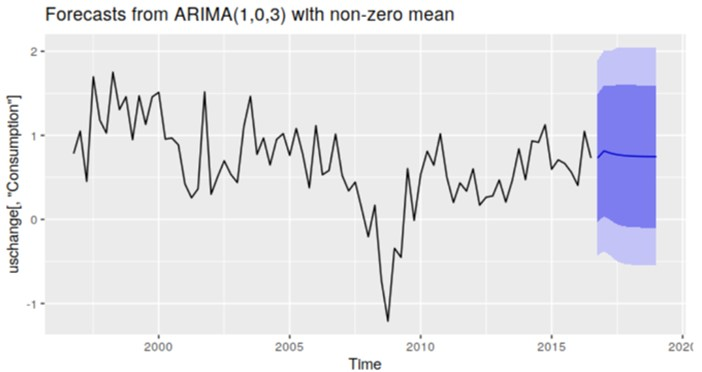
\includegraphics[width=0.7\textwidth]{Imagen12.JPG}
\end{center}
\end{figure}

\end{frame}


%%%%%%%%%%%%%%%%%%%%%%%%%%%%%%%%%%%%%%%%%%%%%%%%%%%%%%%%%%%%




\begin{frame}[fragile]
\frametitle{auto.arima() --> Ojo!}

La función \highlighton{auto.arima()} es útil, pero cualquier cosa automatizada puede ser un poco peligrosa, y vale la pena entender algo sobre el comportamiento de los modelos, incluso cuando confía en un procedimiento automático para elegir el modelo.



\begin{figure}
\begin{center}
    
\includegraphics[width=0.6\textwidth]{Imagen13.JPG}
\end{center}
\end{figure}



\end{frame}


%%%%%%%%%%%%%%%%%%%%%%%%%%%%%%%%%%%%%%%%%%%%%%%%%%%%%%%%%%%%





\subsection{Estimación y selección de orden}

\begin{frame}[fragile]
\frametitle{ACF y PACF}


Por lo general, no es posible saber, simplemente a partir de un diagrama de tiempo, qué valores de $p$ y $q$ son apropiados para los datos. Sin embargo, a veces es posible usar el gráfico \textbf{ACF}, y el gráfico \textbf{PACF} estrechamente relacionado, para determinar los valores apropiados para $p$ y $q$.

\vspace{4mm}

\textbf{Recuerde:}

{\small
\begin{itemize}
\item Un gráfico ACF muestra las autocorrelaciones que miden la relación entre $y_t$ y $y_{t-k}$  para diferentes valores de $k$.
\begin{itemize}
\item Si $y_t$ y $y_{t-1}$ están correlacionados, entonces $y_{t-1}$ y $y_{t-2}$ también deben de estar correlacionados.
\item Entonces $y_t$ y $y_{t-2}$ podrían estar correlacionados, simplemente porque ambos están conectados a $y_{t-1}$, en lugar de cualquier información contenida en $y_{t-2}$ que podría usarse para pronosticar $y_t$
\end{itemize}
 
\end{itemize}
}

\end{frame}


%%%%%%%%%%%%%%%%%%%%%%%%%%%%%%%%%%%%%%%%%%%%%%%%%%%%%%%%%%%%




\begin{frame}[fragile]
\frametitle{ACF y PACF}


Para superar ese problema, podemos usar las \textbf{autocorrelaciones parciales (PACF)}.
\vspace{4mm}

Estos miden la relación entre $y_t$ y $y_{t-k}$ después de eliminar los efectos de los rezagos $1, 2, 3, ..., k-1$.

\vspace{4mm}

\begin{itemize}
\item $\alpha_k$ k-ésima autocorrelación parcial
\item $\alpha_k = \rho_1$: La primera autocorrelación parcial es idéntica a la primera autocorrelación, porque no hay nada entre ellas para eliminar.
\item Cada autocorrelación parcial se puede estimar como el último coeficiente en un modelo autorregresivo.
\item $\alpha_k$ es igual a estimar $\phi_k$ en un $AR(k)$
\end{itemize}


\end{frame}


%%%%%%%%%%%%%%%%%%%%%%%%%%%%%%%%%%%%%%%%%%%%%%%%%%%%%%%%%%%%




\begin{frame}[fragile]
\frametitle{ACF y PACF}


\lstset{language=r,label= ,caption= ,captionpos=b,numbers=none}
\begin{lstlisting}
ggAcf(uschange[,"Consumption"])
ggPacf(uschange[,"Consumption"])
ggtsdisplay(uschange[,"Consumption"])
\end{lstlisting}

\pause


\begin{figure}
\begin{center}
    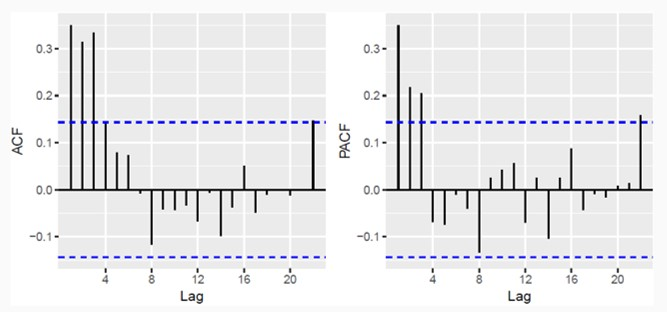
\includegraphics[width=0.8\textwidth]{Imagen14.JPG}
\end{center}
\end{figure}


\end{frame}


%%%%%%%%%%%%%%%%%%%%%%%%%%%%%%%%%%%%%%%%%%%%%%%%%%%%%%%%%%%%



\begin{frame}[fragile]
\frametitle{ACF y PACF}


Los datos pueden seguir un \textbf{ARIMA(p,d,0)} si los gráficos ACF y PACF de los datos diferenciados muestran los siguientes patrones:

\begin{itemize}
\item El ACF es exponencialmente decadente o sinusoidal.
\item Hay un aumento significativo en el rezago $p$ en el PACF, pero ninguno más allá del rezago $p$.
\end{itemize}

\pause
\vspace{4mm}

Los datos pueden seguir un \textbf{ARIMA(0,d,q}) si los gráficos ACF y PACF de los datos diferenciados muestran los siguientes patrones:

\begin{itemize}
\item El PACF es exponencialmente decadente o sinusoidal
\item Hay un aumento significativo en el rezago $q$ en el ACF, pero ninguno más allá del retraso $q$.
\end{itemize}


\end{frame}


%%%%%%%%%%%%%%%%%%%%%%%%%%%%%%%%%%%%%%%%%%%%%%%%%%%%%%%%%%%%




\begin{frame}[fragile]
\frametitle{Ejemplo}


\begin{figure}
\begin{center}
    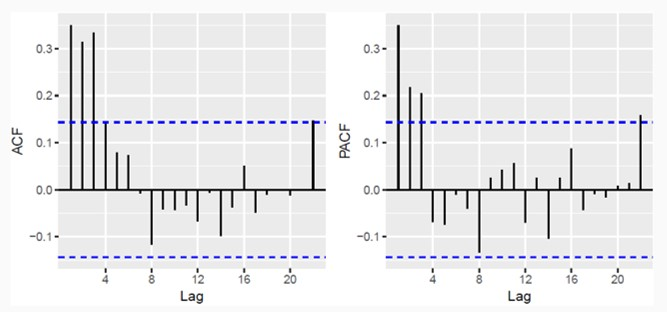
\includegraphics[width=0.5\textwidth]{Imagen14.JPG}
\end{center}
\end{figure}

{\small
\begin{itemize}
\item Hay 3 picos en el ACF, seguidos por un pico casi significativo en el rezago 4. 
\item En el PACF, hay 3 picos significativos, y luego no hay picos significativos después (aparte de uno justo fuera de los límites en rezago 22).
\item Podemos ignorar un pico significativo en cada gráfico si está fuera de los límites, y no en los primeros rezagos.
\item La probabilidad de que un pico sea significativo por casualidad es de aproximadamente 1/20, y estamos trazando 22 picos en cada gráfico.
\end{itemize}
}

\begin{center}
\small \highlighton{El patrón en los primeros 3 picos es lo que esperaríamos de un \textbf{ARIMA(3,0,0)}, ya que el PACF tiende a disminuir.}
\end{center}

\end{frame}


%%%%%%%%%%%%%%%%%%%%%%%%%%%%%%%%%%%%%%%%%%%%%%%%%%%%%%%%%%%%




\begin{frame}[fragile]
\frametitle{Ejemplo}



\lstset{language=r,label= ,caption= ,captionpos=b,numbers=none}
\begin{lstlisting}
fit2 <- Arima(uschange[,"Consumption"], order=c(3,0,0))
\end{lstlisting}

\pause

{\scriptsize
\begin{verbatim}
Series: uschange[, "Consumption"] 
ARIMA(3,0,0) with non-zero mean 

Coefficients:
         ar1     ar2     ar3    mean
      0.2274  0.1604  0.2027  0.7449
s.e.  0.0713  0.0723  0.0712  0.1029

sigma^2 estimated as 0.3494:  log likelihood=-165.17
AIC=340.34   AICc=340.67   BIC=356.5
\end{verbatim}
}


\small Este modelo es en realidad un poco mejor que el modelo identificado por auto.arima(,con un valor AICc de 340.67 en comparación con 342.08. La auto.arima()función no encontró este modelo porque no considera todos los modelos posibles en su búsqueda.

\pause

\lstset{language=r,label= ,caption= ,captionpos=b,numbers=none}
\begin{lstlisting}
fit3 <- auto.arima(uschange[,"Consumption"], seasonal=FALSE,
  stepwise=FALSE, approximation=FALSE)
\end{lstlisting}


\end{frame}


%%%%%%%%%%%%%%%%%%%%%%%%%%%%%%%%%%%%%%%%%%%%%%%%%%%%%%%%%%%%





\begin{frame}[fragile]
\frametitle{Ejemplo}


\lstset{language=r,label= ,caption= ,captionpos=b,numbers=none}
\begin{lstlisting}
fit2 %>% forecast(h=10) %>% autoplot(include=80)
\end{lstlisting}

\pause


\begin{figure}
\begin{center}
    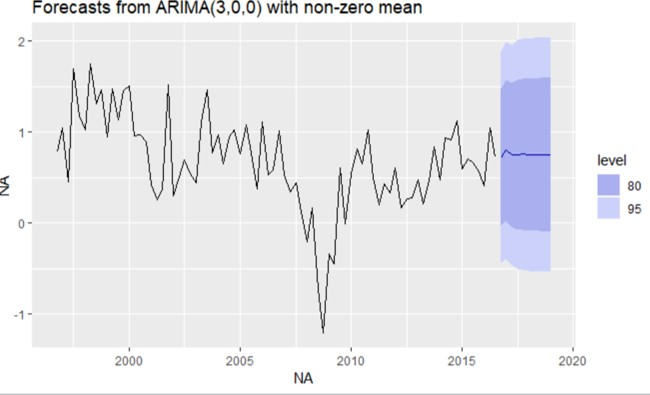
\includegraphics[width=0.8\textwidth]{Imagen15.JPG}
\end{center}
\end{figure}


\end{frame}


%%%%%%%%%%%%%%%%%%%%%%%%%%%%%%%%%%%%%%%%%%%%%%%%%%%%%%%%%%%%




\begin{frame}[fragile]
\frametitle{Criterios de información}


\begin{itemize}
\item AIC
\item AICc
\item BIC
\end{itemize}

\vspace{4mm}

Buenos modelos son obtenidos minimizando los criterios: AIC, AICc, BIC.

\vspace{4mm}

Es importante tener en cuenta que estos criterios de información tienden a no ser buenas guías para seleccionar el orden apropiado de diferenciación $(d)$ de un modelo, sino solo para seleccionar los valores de $p$ y $q$.

\vspace{4mm}

La diferenciación cambia los datos en los que se calcula la probabilidad, lo que hace que los valores de AIC entre modelos con diferentes órdenes de diferenciación no sean comparables.

\end{frame}


%%%%%%%%%%%%%%%%%%%%%%%%%%%%%%%%%%%%%%%%%%%%%%%%%%%%%%%%%%%%





\begin{frame}[fragile]
\frametitle{Procedimiento de modelado}


Al ajustar un modelo ARIMA a un conjunto de datos de series temporales (no estacionales), el siguiente procedimiento proporciona un enfoque general.

{\small
\begin{enumerate}
\item Trace los datos e identifique cualquier observación inusual.
\item Si es necesario, transforme los datos (usando una transformación Box-Cox) para estabilizar la varianza.
\item Si los datos no son estacionarios, tome las primeras diferencias de los datos hasta que los datos sean estacionarios.
\item Examine la ACF / PACF
\item Pruebe los modelos elegidos y use el AICc para buscar un modelo mejor.
\item Verifique los residuos de su modelo elegido trazando el ACF de los residuos y haciendo una prueba de resumen de los residuos. Si no parecen ruido blanco, pruebe con un modelo modificado.
\item Una vez que los residuos se vean como ruido blanco, calcule los pronósticos.
\end{enumerate}
}

\end{frame}


%%%%%%%%%%%%%%%%%%%%%%%%%%%%%%%%%%%%%%%%%%%%%%%%%%%%%%%%%%%%





\begin{frame}[fragile]
\frametitle{Ejemplo}


Aplicaremos este procedimiento a los datos de pedidos de equipos eléctricos ajustados estacionalmente.



\lstset{language=r,label= ,caption= ,captionpos=b,numbers=none}
\begin{lstlisting}
elecequip %>% stl(s.window='periodic') %>% seasadj() -> eeadj
autoplot(eeadj)
\end{lstlisting}

\pause


\begin{figure}
\begin{center}
    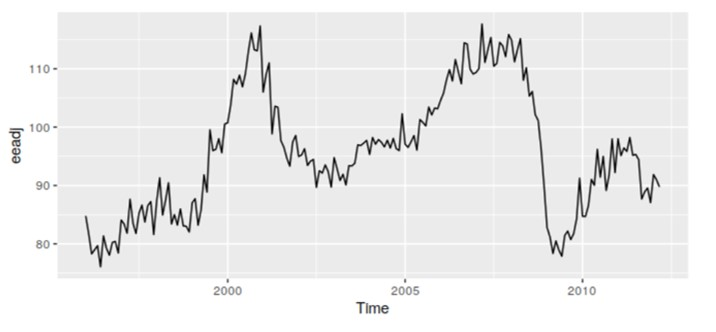
\includegraphics[width=0.8\textwidth]{Imagen16.JPG}
\end{center}
\end{figure}




\end{frame}


%%%%%%%%%%%%%%%%%%%%%%%%%%%%%%%%%%%%%%%%%%%%%%%%%%%%%%%%%%%%




\begin{frame}[fragile]
\frametitle{Ejemplo}


\begin{itemize}
\item El diagrama de tiempo muestra algunos cambios repentinos, particularmente la gran caída en 2008/2009. Estos cambios se deben al entorno económico mundial. De lo contrario, no hay nada inusual en el diagrama de tiempo y parece que no hay necesidad de hacer ningún ajuste de datos.
\vspace{3mm}

\item No hay evidencia de cambios en la varianza, por lo que no haremos una transformación de Box-Cox.
\vspace{3mm}
\item Los datos son claramente no estacionarios, ya que la serie se desplaza hacia arriba y hacia abajo durante largos períodos. 
\end{itemize}

\end{frame}


%%%%%%%%%%%%%%%%%%%%%%%%%%%%%%%%%%%%%%%%%%%%%%%%%%%%%%%%%%%%





\begin{frame}[fragile]
\frametitle{Ejemplo}


\lstset{language=r,label= ,caption= ,captionpos=b,numbers=none}
\begin{lstlisting}
eeadj %>% diff() %>% ggtsdisplay(main="")
\end{lstlisting}

\pause

\begin{figure}
\begin{center}
    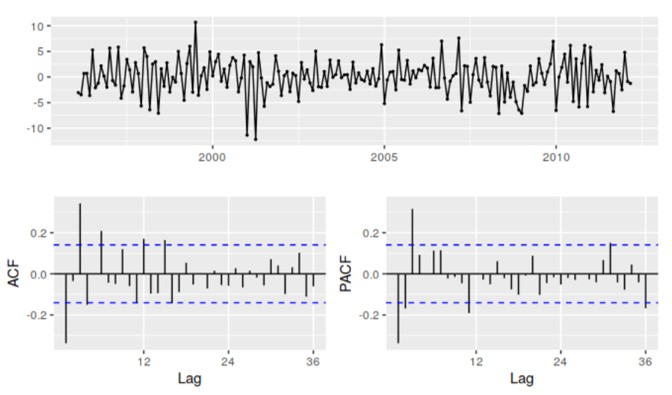
\includegraphics[width=0.8\textwidth]{Imagen17.JPG}
\end{center}
\end{figure}


\end{frame}


%%%%%%%%%%%%%%%%%%%%%%%%%%%%%%%%%%%%%%%%%%%%%%%%%%%%%%%%%%%%




\begin{frame}[fragile]
\frametitle{Ejemplo}


\begin{itemize}
\item El PACF que se muestra sugiere un modelo AR(3). Entonces, un modelo candidato inicial es un ARIMA (3,1,0). No hay otros modelos candidatos obvios.

\vspace{3mm}

\item Ajustamos un modelo ARIMA(3,1,0) junto con variaciones que incluyen ARIMA(4,1,0), ARIMA(2,1,0), ARIMA(3,1,1), etc. De estos, el ARIMA(3,1,1) tiene un valor AICc ligeramente menor. 
\end{itemize}

\end{frame}


%%%%%%%%%%%%%%%%%%%%%%%%%%%%%%%%%%%%%%%%%%%%%%%%%%%%%%%%%%%%





\begin{frame}[fragile]
\frametitle{Ejemplo}



\lstset{language=r,label= ,caption= ,captionpos=b,numbers=none}
\begin{lstlisting}
fit <- Arima(eeadj, order=c(3,1,1))
\end{lstlisting}

\pause

{\scriptsize
\begin{verbatim}
Series: eeadj 
ARIMA(3,1,1) 

Coefficients:
         ar1     ar2     ar3      ma1
      0.0044  0.0916  0.3698  -0.3921
s.e.  0.2201  0.0984  0.0669   0.2426

sigma^2 estimated as 9.577:  log likelihood=-492.69
AIC=995.38   AICc=995.7   BIC=1011.72
\end{verbatim}
}


\end{frame}


%%%%%%%%%%%%%%%%%%%%%%%%%%%%%%%%%%%%%%%%%%%%%%%%%%%%%%%%%%%%




\begin{frame}[fragile]
\frametitle{Ejemplo}


\small El gráfico ACF de los residuos del modelo ARIMA(3,1,1) muestra que todas las autocorrelaciones están dentro de los límites del umbral, lo que indica que los residuos se comportan como el ruido blanco. Una prueba de portmanteau devuelve un valor p grande, lo que también sugiere que los residuos son ruido blanco.

\lstset{language=r,label= ,caption= ,captionpos=b,numbers=none}
\begin{lstlisting}
checkresiduals(fit)
\end{lstlisting}

\pause


\begin{figure}
\begin{center}
    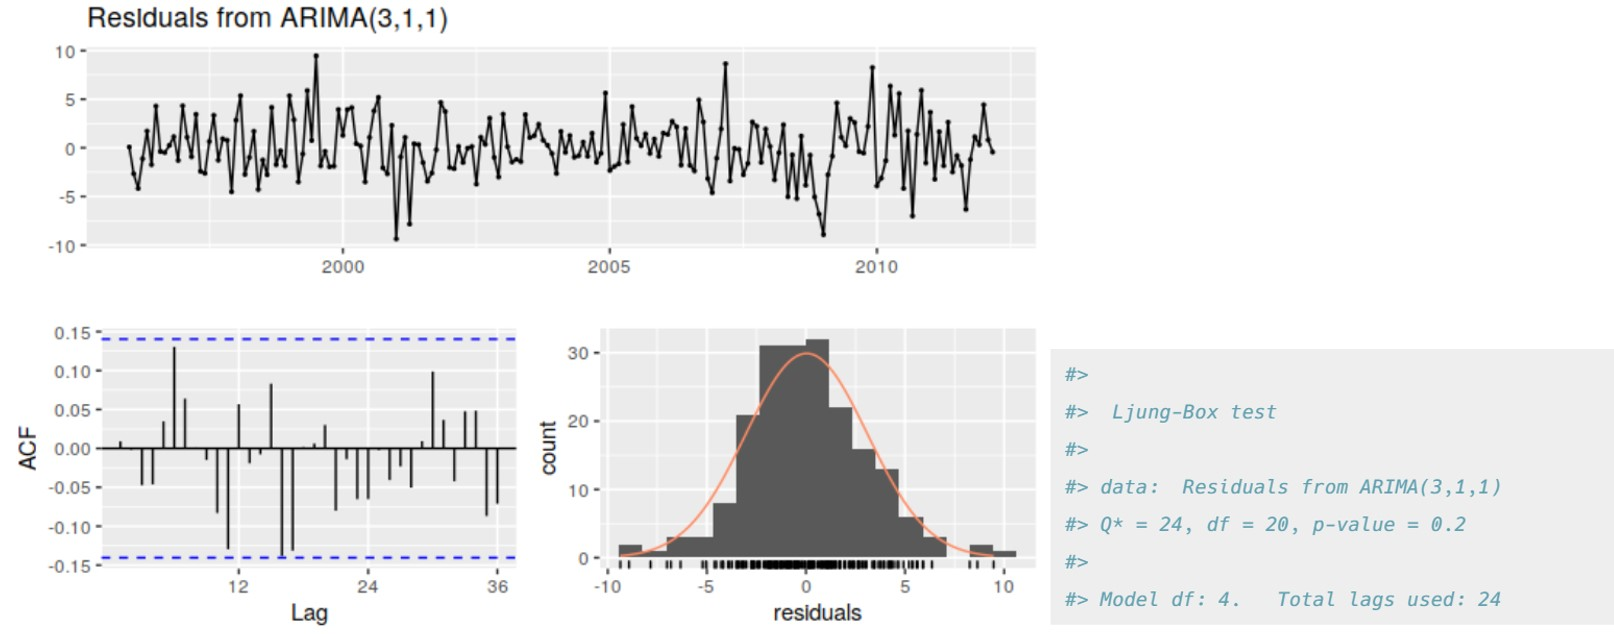
\includegraphics[width=0.8\textwidth]{Imagen18.JPG}
\end{center}
\end{figure}

\end{frame}


%%%%%%%%%%%%%%%%%%%%%%%%%%%%%%%%%%%%%%%%%%%%%%%%%%%%%%%%%%%%




\begin{frame}[fragile]
\frametitle{Ejemplo}


\lstset{language=r,label= ,caption= ,captionpos=b,numbers=none}
\begin{lstlisting}
autoplot(forecast(fit))
\end{lstlisting}

\pause


\begin{figure}
\begin{center}
    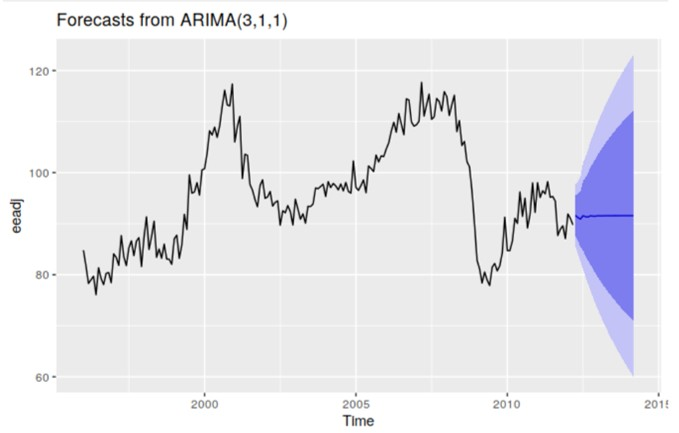
\includegraphics[width=0.7\textwidth]{Imagen19.JPG}
\end{center}
\end{figure}

\end{frame}


%%%%%%%%%%%%%%%%%%%%%%%%%%%%%%%%%%%%%%%%%%%%%%%%%%%%%%%%%%%%




\begin{frame}[fragile]
\frametitle{Ejemplo}


\lstset{language=r,label= ,caption= ,captionpos=b,numbers=none}
\begin{lstlisting}
autoplot(fit)
\end{lstlisting}

\pause


\begin{figure}
\begin{center}
    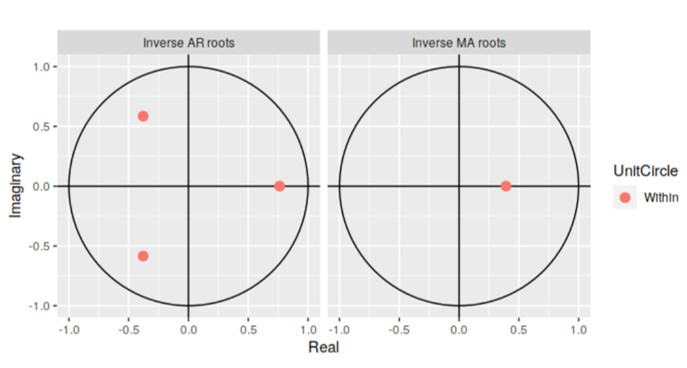
\includegraphics[width=0.7\textwidth]{Imagen20.JPG}
\end{center}
\end{figure}


\small Los tres puntos rojos en la gráfica de la izquierda corresponden a las raíces de los polinomios $\phi(B)$, mientras que el punto rojo en la gráfica de la derecha corresponde a la raíz de $\theta(B)$. Todos están dentro del círculo unitario, como es de esperar, porque R asegura que el modelo ajustado sea tanto estacionario como invertible.


\end{frame}


%%%%%%%%%%%%%%%%%%%%%%%%%%%%%%%%%%%%%%%%%%%%%%%%%%%%%%%%%%%%



%%%%%%%%%%%%%%%%%%%%%%%%%%%%%%%%%%%%%%%%%%%%%%%%%%%%%%%%%%%%



%%%%%%%%%%%%%%%%%%%%%%%%%%%%%%%%%%%%%%%%%%%%%%%%%%%%%%%%%%%%



%%%%%%%%%%%%%%%%%%%%%%%%%%%%%%%%%%%%%%%%%%%%%%%%%%%%%%%%%%%%








%%%%%%%%%%%%%%%%%%%%%%%%%%%%%%%%%%%%%%%%%%%%%%%%%%%%%%%%%%%%%%%%%%%%%%%











%%%%%%%%%%%%%%%%%%%%%%%%%%%%%%%%%%%%%%%%%%%%%%%%%%%%%%%%%%%%%%%%%%%%% 




\frame{
  \vspace{2cm}
  {\huge Preguntas?}


\vspace{2.5cm}

\begin{flushright}
\highlighton{
  \usebeamerfont*{frametitle}Gracias!!},
\end{flushright}

  
  \begin{flushright}
    Jr.
    
   \structure{\footnotesize{orlando.joaqui@correounivalle.edu.co}}
  \end{flushright}
}







\end{document}
